\section{Level Converter}
The purpose of this block is to supply both the Load System and the Control Unit with 5 VDC. This is done by converting the 12 VDC from the Voltage Adaptor's output.

\subsection{Design}
The block is supplied by 12 VDC from the Voltage Adaptor. This voltage-level is converted to 5 VDC using a LM7805 voltage regulator. In order to give a steady DC-output, the voltage regulator is set up as shown on figure \ref{fig:LM7805_app} seen below.

\begin{figure}[H]
	\centering
	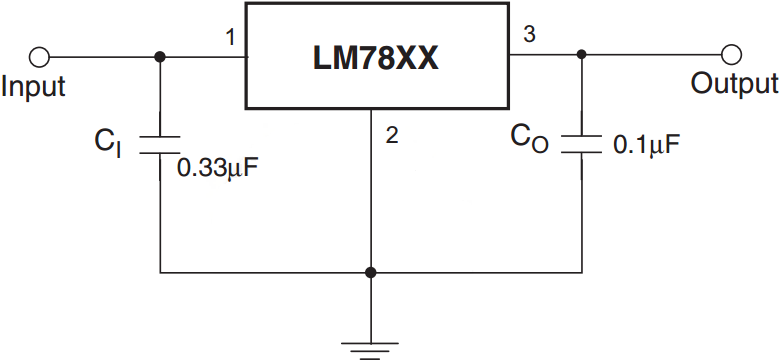
\includegraphics[width=0.5\linewidth]{Hardware/Pictures/LM7805}
	\caption{DC application for LM7805}
	\label{fig:LM7805_app}
\end{figure}

\subsection{Implementation}
The circuit is built identically as the one seen in the reguulator's application note. However, a 1 Amp fuse has been connected to the output in order to protect the supplied circuits from a possible over-current.

\subsection{Unity test}
Text